\documentclass[page number]{beamer}
\usetheme[sectionpage=none,numbering=fraction,progressbar=foot]{metropolis}
\usepackage{etex}
\usepackage{graphicx, booktabs} % For tabulars
\usepackage{pgf,tikz}
\usepackage{ulem}
\usetikzlibrary{arrows}
\usetikzlibrary{positioning,shapes,fit}
\usepackage{algorithm}
\usepackage{algpseudocode}
\usepackage{multicol}
\usepackage{syntax}
\usepackage{xcolor, color, colortbl}
\usepackage{tikz-qtree}
\usepackage{listings}
\usepackage{mathtools}
\usepackage{amssymb}
\usepackage{amsmath}

\makeatletter
\makeatother

%\setcounter{tocdepth}{1} % remove subsection from table of contents

% colors
\definecolor{mDarkRed}{HTML}{6F1616}
\definecolor{mDarkGreen}{HTML}{106235}
\definecolor{mTeal}{HTML}{112233}
\definecolor{mBlack}{HTML}{000000}
\setbeamercolor{normal text}{fg=mTeal}
\setbeamercolor{alerted text}{fg=mDarkRed}
\setbeamercolor{example text}{fg=mDarkGreen}
\setbeamercolor{title separator}{fg=purple,bg=mBlack}

% macros
\def\ctls{CTL$^{*}$}
\def\ctlskd{CTL$^{*}$K$\Delta$}
\def\ctlskdp{CTL$^{*}$K$\Delta\psi$}
\def\ap{AP}
\def\A{\mathit{A}}
\def\E{\mathit{E}}
\def\U{\mathit{U}}
\def\R{\mathit{R}}
\def\X{\mathit{X}}
\def\K{\mathit{K}}
\def\KP{\bar{\mathit{K}}}
\def\D#1{\Delta^{#1}}
\def\eq#1#2{\approx^{#2}_{#1}}
\def\eqh#1{\approx_{#1}}
\def\eqstate#1{\sim_{#1}}
\def\todo#1{{\color{red}#1}}
\def\iff{\ \mathit{iff}\ }
\def\UD{U_{\Delta}}
\def\UT{U_T}
\def\UDK#1{U_{\Delta #1}}
\def\UTK#1{U_{T #1}}
\def\FV{\mathit{FH}}
\def\FP{\mathit{FP}}
\def\ktree{$k$-tree}
\def\ktrees{$k$-trees}
\def\outline{
  \begin{frame}[plain,noframenumbering]
    \frametitle{Outline}
    \tableofcontents[currentsection]
  \end{frame}
}


\begin{document}
\title[\ctlskd]{Defining and Model-Checking an Epistemic Temporal Logic with Changes of Observations}

\author[Aur\`ele Barri\`ere]{Aur\`ele Barri\`ere\hfill\textbf{Supervisors:}\begin{tabular}{c}
    Aniello Murano\\
    Bastien Maubert\\
    Sasha Rubin\\
  \end{tabular}}
% add supervisors
\date{\textit{ENS Rennes\hfill Universit\`a degli Studi di Napoli Federico II}
  \vfill
  \textbf{January 8, 2018}}

\def\outline{
  \begin{frame}[plain,noframenumbering]
    \frametitle{Outline}
    \tableofcontents[currentsection]
  \end{frame}
}

\begin{frame}[plain,noframenumbering]
  \vspace{-2cm}
  \maketitle
  \vspace{-4cm}
\end{frame}

\metroset{sectionpage=none}
\section{Introduction}
\begin{frame}{Temporal Logics}

  \begin{block}{Evolving Systems}
    Typically modelled wih \textbf{Kripke Structures} $M=(S,I,T,V)$.\\

    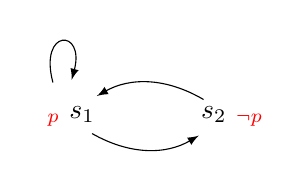
\begin{tikzpicture}[%
        every node/.style={circle,minimum size=4pt,minimum height=4pt, inner sep=0pt},
        shorten >=2pt,
        node distance=1.3cm, >=latex
      ]
      \node [] (0) [circle] {$~_{\color{red}~ p}~s_{1}$};
      \node [] (1) [circle, right=of 0] {$s_{2}~_{\color{red}\neg p}$}; 
      \path [draw] (0) edge[->, bend right]  node {} (1)
      (0) edge[->, loop above]  node {} (0)
      (1) edge[->, bend right]  node {} (0);
    \end{tikzpicture}\hfill
    \begin{tabular}{c l l}
      $S$ & States &\\
      $I$ & Initial states & $\subseteq S$\\
      $T$ & Transitions & $\subseteq S\times S$\\
      $V$ & Valuation & $S\rightarrow 2^{AP}$
    \end{tabular}
  \end{block}
  \vfill
  \begin{block}{Temporal Logics}
    \begin{tabular}{l c r}
    Syntax & defines & $\varphi$\\
    Semantics & defines & $M\models\varphi$
    \end{tabular}
  \end{block}
  \vfill
  \begin{block}{Model-Checking}
    Given Kripke Structure $M$, and formula $\varphi$, does $M\models\varphi$?
  \end{block}
  
\end{frame}


\begin{frame}{A Temporal Logic: \ctls}

  \begin{block}{Syntax}
    \begin{tabular}{l l}
      State formulas & $\varphi := p ~|~ \neg \varphi ~|~ \varphi\wedge\varphi ~|~ \A\psi$\\
      Path formulas & $\psi := \varphi ~|~ \neg\psi ~|~ \psi\wedge\psi ~|~ \X\psi ~|~ \psi\U\psi$\\
    \end{tabular}
    
      $\A:$ for all paths\hfill
      $\X:$ next\hfill
      $\U:$ until\hfill
  \end{block}
  \vfill
  \begin{block}{Semantics}
    \begin{tabular}{l c l}
      $M,s \models p $&$ \iff $&$ p\in V(s)$\\
      $M,s \models \A\psi  $&$ \iff $&$ \forall\pi$ that starts in $s$, we have $M,\pi\models\psi$\\
      $M,\pi\models\varphi $&$ \iff $&$ M,\mathit{last}(\pi)\models\varphi$\\
      $M,\pi\models\X\psi $&$ \iff $&$  M,\pi_{> 0}\models\psi$\\
      $M,\pi\models\psi_1\U\psi_2 $&$ \iff $&$ \exists m\geq 0$ such that $\forall k\in[0,m[, M,\pi_{\geq k}\models\psi_1$\\
          & & and $M,\pi_{\geq m}\models\psi_2$\\
          \hline
      $M\models\varphi$&$ \iff $&$\forall s\in I, \quad M,s\models\varphi$
\end{tabular}
  \end{block}
  
\end{frame}


\begin{frame}{Model Checking}

  \begin{block}{Exemple}
    \begin{center}
     \begin{tikzpicture}[%
        every node/.style={circle,minimum size=4pt,minimum height=4pt, inner sep=0pt},
        shorten >=2pt,
        node distance=0.6cm, >=latex
      ]
      \node [] (0) [circle] {$s_{1}$};
      \node [] (1) [circle, below right=of 0] {$s_{2}$};
      \node [] (2) [circle, below left=of 0] {$s_{3}$};
      \node [] (3) [circle, below right=of 2] {$s_{4}~_{\color{red}p}$};
      \node [] (4) [circle, above=of 0] {};
      \node [] (5) [rectangle, right=of 1,xshift=1cm] {$\varphi=\A\X\X p$};      
      \path [draw] (0) edge[->]  node {} (1)
      (1) edge[->]  node {} (3)
      (0) edge[->]  node {} (2)
      (2) edge[->]  node {} (3)
      (4) edge[->]  node {} (0);
     \end{tikzpicture}
    \end{center}
     For every possible path starting in $s_1$, $p$ is true after two steps.
  \end{block}
  \vfill
  \begin{exampleblock}{Model Checking of \ctls\ is decidable}
    Complexity PSPACE.
  \end{exampleblock}
  
\end{frame}


\begin{frame}{Epistemic Logics}

  \begin{block}{Multi-agent systems and Imperfect Information}
    Agents each have an observation (equivalence relation on states).
    \vspace{-0.4cm}
    \begin{center}
    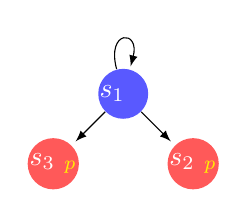
\begin{tikzpicture}[%
        every node/.style={circle,minimum size=4pt,minimum height=4pt, inner sep=0pt},
        shorten >=2pt,
        node distance=0.6cm, >=latex
      ]
      \node [] (0) [circle, fill=blue!65] {$\color{white}s_{1}~_{\hphantom{p}}$};
      \node [] (1) [circle, below right=of 0, fill=red!65] {$\color{white}s_{2}~_{\color{yellow}p}$};
      \node [] (2) [circle, below left=of 0, fill=red!65] {$\color{white}s_{3}~_{\color{yellow}p}$};
      \path [draw] (0) edge[->]  node {} (1)
      (0) edge[->, loop above]  node {} (0)
      (0) edge[->]  node {} (2);
    \end{tikzpicture}
    \quad\quad\quad
    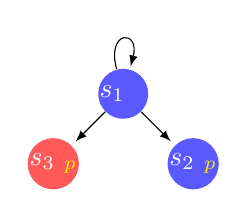
\begin{tikzpicture}[%
        every node/.style={circle,minimum size=4pt,minimum height=4pt, inner sep=0pt},
        shorten >=2pt,
        node distance=0.6cm, >=latex
      ]
      \node [] (0) [circle, fill=blue!65] {$\color{white}s_{1}~_{\hphantom{p}}$};
      \node [] (1) [circle, below right=of 0, fill=blue!65] {$\color{white}s_{2}~_{\color{yellow}p}$};
      \node [] (2) [circle, below left=of 0, fill=red!65] {$\color{white}s_{3}~_{\color{yellow}p}$};
      \path [draw] (0) edge[->]  node {} (1)
      (0) edge[->, loop above]  node {} (0)
      (0) edge[->]  node {} (2);
    \end{tikzpicture}
    \end{center}
    \vspace{-0.4cm}    
  \end{block}
  \vfill
  \begin{block}{Knowledge operator}
    \begin{tabular}{r l}
      $\K_a p$ : & Agent $a$ knows that $p$ holds.\\
      $\K_a\K_b p$ : & Agent $a$ knows that agent $b$ knows $p$.
    \end{tabular}
  \end{block}
  \vfill
  \begin{exampleblock}{Epistemic Temporal Logics}
    System goes through $(s_1,s_2)$.\\
    \begin{tabular}{l l}
    Possible histories for & agent 1: $(s_1,s_2)$ and $(s_1,s_3)$.\\
                           & agent 2: $(s_1,s_2)$ and $(s_1,s_1)$.
    \end{tabular}\\
    Only the first agent knows that $p$ holds.
  \end{exampleblock}
  
\end{frame}


\begin{frame}{Strategy Logic with Imperfect Information}

  \begin{block}{A logic for strategies in multi-agent systems}
    $\left<\left< x\right>\right>^o~(a,x)~\varphi$~:\quad
    There exists a strategy $x$ with observation $o$, such that if agent $a$ uses $x$, $\varphi$ holds.
  \end{block}
  \vfill
  \begin{alertblock}{Changes of observation}
    $\left<\left< x\right>\right>^o\left<\left< y \right>\right>^{o'}~(a,x)~\X~(a,y)~\varphi$
  \end{alertblock}
  \vfill
  \begin{exampleblock}{Towards an epistemic extension of SLii}
    How do changes of observations and epistemic operators interact?
  \end{exampleblock}
    
\end{frame}


\begin{frame}{\ctlskd}

  \begin{block}{An Epistemic Temporal Logic with Changes of Observation}
    \begin{itemize}
    \item Branching-time Temporal Operators $\X,\U,\A$.
    \item Knowledge Operator $\K$.
    \item Dedicated operator for change of observation $\D{o}$.
    \item Synchronous Perfect-Recall Semantics.
    \end{itemize}
  \end{block}
  \vfill
  \begin{exampleblock}{Objectives}
    \begin{itemize}
    \item Define \ctlskd\ for the single-agent setting.
    \item Solve the model-checking problem.
    \item Extend logic and model-checking to the multi-agent setting.
    \end{itemize}
  \end{exampleblock}
  
\end{frame}


\metroset{sectionpage=progressbar}
\section{\ctlskd: Single Agent}
\subsection{Syntax}

We begin by introducing the syntax of our logic. It contains operators of branching-time logics, temporal logics and epistemic logics, as well as a new one to indicate changes of observations. At first, we will study the case where there is only one agent (and thus only one  knowledge operator).

We consider $\mathcal{O}$ to be a set of \textit{observations}, that each represent a possible observational power of the agent. $\mathit{AP}$ is a set of atomic propositions.
Formulas of \ctlskd\ can be \textit{history formulas} $\varphi$ or \textit{path formulas} $\psi$.

$$\varphi := p ~|~ \neg \varphi ~|~ \varphi\wedge\varphi ~|~ \A\psi ~|~ \K\varphi ~|~ \D{o}\varphi$$
$$\psi := \varphi ~|~ \neg\psi ~|~ \psi\wedge\psi ~|~ \X\psi ~|~ \psi\U\psi$$

Where $p\in\mathit{AP}$ and $o\in\mathcal{O}$.
The temporal operators $\X$ and $\U$ are meant to represent the typical \textit{next} and \textit{until} operators of temporal logics.
$\A$ is a path quantifier, similar to those found in branching-time logics. Intuitively, $\A\psi$ should hold for a history if $\psi$ is true in every possible future.
$\K$ is an epistemic operator. Intuitively, $\K\varphi$ should be true whenever the agent knows that $\varphi$ is true. We introduce a new one, $\D{o}$, to represent a change of observation.
$\varphi$ is called a history formula, as we only need to know what happened in the past to decide if the formula is true. $\psi$ is called a path formula as it also requires the future evolution of the system.

We can also define the temporal operator $\R$ (the \textit{release}), dual of $\U$. The path quantifier $\E$, dual of $\A$. The knowledge operator $\KP$ (\textit{possibility}), dual of $\K$. With negation and $\wedge$, we can also define the classical Boolean operators $\vee$ and $\rightarrow$.

\subsection{Semantics}

The models on which such formulas can be interpreted are classical Kripke Structure, with several equivalence relations between states (one for each observation).
Let $\mathcal{O}=\{o_1,o_2,\dots,o_m\}$.
A Kripke Structure with observations is a structure $M=(S,I_s,o_I,T,V,\eqstate{o_1},\dots,\eqstate{o_m})$ where

\begin{tabular}{r l}
$S$& is a set of states.\\
$I_s\subseteq S$& is a set of initial states.\\
$o_I$& is the initial observation.\\
$T\subseteq S\times S$& is a transition relation between states.\\
$V:S\rightarrow 2^{\mathit{AP}}$& is a valuation function.\\
$\forall o_i, \eqstate{o_i}$& is an equivalence relation between states.
\end{tabular}

A \textit{run} or \textit{path} is an infinite sequence of states $\pi=\pi_0\pi_1\dots$. A \textit{history} is a finite sequence of states $h=h_1\dots h_n$.

\subsubsection{Observation records}
Given $\mathcal{O}$ a set of observations, we define \textit{observations records} to be ordered lists of pairs of observations and natural numbers.
Intuitively, an observation record represents changes of observations.

\textbf{Example:}  $r=[(o_1,0),(o_2,3),(o_3,3)]$ means that the player starts at time 0 with observation $o_1$. It keeps this observation, then at time 3, it first changes to $o_2$ and then to $o_3$. We use observation records in the semantics to remember the previous observations of the agent.

We write $r[(o,n)]$ to append a new pair $(o,n)$ to the observation record $r$.
We write $r_{\leq n}$ the record $r$ without the pairs $(o,m)$ where $m>n$.
We write $r_n$ the record $r$ without the pairs $(o,m)$ where $m\neq n$. 
We define a function $\mathit{O}(r,n)$ which gives a tuple of the observations at time $n$. $\mathit{O}(r,n)$ includes every observation of $r_n$, as well as the previous one.

\textbf{Example:} Let $r=[(o_1,0),(o_2,3),(o_3,3)]$. $\mathit{O}(r,0)=(o_I,o_1), \mathit{O}(r,1)=\mathit{O}(r,2)=(o_1)$, $\mathit{O}(r,3)=(o_1,o_2,o_3)$ and $\mathit{O}(r,4)=(o_3)$.

On a given model, with an observation record we can define an equivalence relation between histories (finite sequences of states), with regard to a record. Two histories are equivalent with regard to the record if the player can't distinguish them by using the observations in the record.\\
$h\eqh{r}h'\quad\iff\quad \forall i< |h|, \forall o\in \mathit{O}(r,i), h(i)\eqstate{o} h'(i)~\textit{and}~|h|=|h'|.$

\subsubsection{Record semantics}
We first define the intuitive semantics of \ctlskd. History formulas need a history $h$ (finite sequence of previous states) and an observation record $r$ to be interpreted, to know which history might be considered possible for the agent.
Path formulas are interpreted on a run $\pi$ (infinite sequence of states of the model), a point in time (natural number), and an observation record.

\begin{tabular}{l c l}
  $M,h,r \models p $&$ \iff $&$ p\in V(\mathit{last}(h))$\\
  $M,h,r \models \neg\varphi $&$ \iff $&$ M,h,r\not\models\varphi$\\
  $M,h,r \models \varphi_1\wedge\varphi_2 $&$ \iff $&$ (M,h,r\models\varphi_1~\text{and}~ M,h,r\models\varphi_2)$\\
  $M,h,r \models \A\psi  $&$ \iff $&$ \forall\pi$ that extends $h$, we have $M,\pi,|h|-1,r\models\psi$\\
  $M,h,r \models\K\varphi  $&$ \iff $&$ \forall h'$ such that $h'\eqh{r}h$, we have $M,h',r\models\varphi$\\
  $M,h,r \models \D{o}\varphi $&$ \iff $&$ M,h,r[(o,|h|-1)]\models\varphi$\\
  $M,\pi,n,r\models\varphi $&$ \iff $&$ M,(\pi_0\dots\pi_n),r\models\varphi$\\
  $M,\pi,n,r\models\neg\psi $&$ \iff $&$ M,\pi,n,r\not\models\psi$\\
  $M,\pi,n,r\models \psi_1\wedge\psi_2 $&$ \iff $&$ (M,\pi,r,n\models\psi_1~\text{and}~ M,\pi,r,n\models\psi_2)$\\
  $M,\pi,n,r\models\X\psi $&$ \iff $&$  M,\pi,(n+1),r\models\psi$\\
  $M,\pi,n,r\models \psi_1\U\psi_2 $&$ \iff $&$ \exists m\geq n$ such that $\forall k\in[n,m[, M,\pi,k,r\models\psi_1$\\
   & & and $M,\pi,m,r\models\psi_2$
\end{tabular}

Finally, we say that $M=(S,I_s,o_I,T,V,\eqstate{o_1},\dots,\eqstate{o_m})$ models $\varphi$ (written $M\models\varphi$), if $\forall s\in I_s, M,s,[(o_I,0)]\models\varphi$. This definition corresponds to the model-checking problem that we solve in Section~\ref{sec:mc}.

\subsubsection{A few validities of \ctlskd}~

\begin{tabular}{l r}
$\D{o}(\varphi_1\wedge\varphi_2)\quad\leftrightarrow\quad(\D{o}\varphi_1\wedge\D{o}\varphi_2)$ & (distributivity)\\
$\D{o}\neg\varphi\quad\leftrightarrow\quad\neg\D{o}\varphi$ & (self-duality)\\
$\D{o}\A\X\D{o}\K\varphi\quad\leftrightarrow\quad\D{o}\A\X\K\varphi$ & (redundant change of observation)\\
$\D{o}\K\varphi\quad\rightarrow\quad\D{o}\K\D{o}\K\varphi$ & (positive introspection)
\end{tabular}

\subsubsection{Our Model-Checking approach}
Once \ctlskd\ is defined, our goal is to solve the model-checking problem. Because of perfect-recall semantics, it may seem that we have to remember the complete history and records when evaluating a formula. However, our main idea is that we can extract some information from the history that is sufficient for the evaluation of the formula. Intuitively, to evaluate a history formula, it is enough to know the current state, the current observation and the set of states that the agent believes the system might be in (this set is later called the \textit{Information Set}). This new structure to represent the knowledge is more succinct than remembering entire histories and records, as there is a finite number of information sets.
We start by defining a new semantics for the same formulas. This semantics uses information sets. Then, we will present an algorithm to model-check a formula according to these new semantics.

\section{Alternative Semantics}
\begin{frame}{Information Sets}

  \begin{block}{Information Sets}
    The set of states that the agent believes the system might be in.
  \end{block}
  \vfill
  \begin{block}{Updating information Sets}
    \begin{tabular}{r c c c l}
    $\UD(I,s,o)$& = &$\{x\in I$ & $~|~$ & $x\eqstate{o}s\}$\\
    $\UT(I,s,o)$& = &$\{x\in S$ & $~|~$ & $\exists t\in I, t\rightarrow x ~\text{and}~ x\eqstate{o}s\}$\\
    \end{tabular}
    
    $\UD(I,s,o)$ When changing to observation $o$ in state $s$ with Information set $I$.\\
    $\UT(I,s,o)$ When going to state $s$ with observation $o$ and Information set $I$.
  \end{block}
\end{frame}

\begin{frame}{Defining Alternative Semantics}
  \footnotesize
  \begin{block}{Alternative Semantics}
    \begin{tabular}{l c l}
      $M,s,I,o\models p $&$ \iff $&$ p\in V(s)$\\
      $M,s,I,o\models\neg\varphi $&$ \iff $&$ M,s,I,o\not\models\varphi$\\
      $M,s,I,o\models \varphi_1\wedge\varphi_2 $&$ \iff $&$ (M,s,I,o\models\varphi_1~\text{and}~M,s,I,o\models\varphi_2)$\\
      $M,s,I,o\models\A\psi $&$ \iff $&$ \forall\pi$ such that $\pi_0=s$, we have $M,\pi,I,o\models\psi$\\
      \color{red!85!blue}$M,s,I,o\models\K\varphi $&$ \iff $&\color{red!85!blue}$ \forall s'\in I$, we have $M,s',I,o\models\varphi$\\
      \color{red!85!blue}$M,s,I,o'\models\D{o}\varphi $&$ \iff $&\color{red!85!blue}$ M,s,\UD(I,s,o),o\models\varphi$\\
      $M,\pi,I,o\models\varphi $&$ \iff $&$ M,\pi_0,I,o\models\varphi$\\
      $M,\pi,I,o\models\neg\psi $&$ \iff $&$ M,\pi,I,o\not\models\psi$\\
      $M,\pi,I,o\models\psi_1\wedge\psi_2 $&$ \iff $&$ (M,\pi,I,o\models\psi_1~\text{and}~M,\pi,I,o\models\psi_2)$\\
      \color{red!85!blue}$M,\pi,I,o\models\X\psi $&$ \iff $&\color{red!85!blue}$ M,\pi_{1\dots},\UT(I,\pi_1,o),o\models\psi$\\
      $M,\pi,I,o\models\psi_1\U\psi_2 $&$ \iff $&$ \exists n\geq 0$, $\forall m\leq n, M,\pi_{m\dots},\UT^m(I,\pi,o),o\models\psi_1$ and\\
      & & $M,\pi_{n\dots},\UT^n(I,\pi,o),o\models\psi_2$
    \end{tabular}
  \end{block}
  \vfill
  \begin{block}{~}
    \begin{center}
    \begin{tabular}{l l | l l}
      $s$ & Current state & $o$ & Current Observation\\
      $I$ & Information set & $\pi$ & Future states, starting in the current one\\
    \end{tabular}
    \end{center}
  \end{block}
\end{frame}
  
\begin{frame}{Reduction Theorem}

  \begin{block}{Extracting Information Sets}
    From a history and a record, we can get the corresponding Information set, current set and observation. $\FV(h,r)=(s,I,o)$.
  \end{block}
  \vfill
  \begin{block}{Reduction Theorem}
    $\forall\varphi$ history formula of \ctlskd, $\forall h,r,s,I,o$ such that\\ $\FV(h,r)=(s,I,o)$, \quad$M,h,r\models\varphi\iff M,s,I,o\models\varphi$.
  \end{block}
  \vfill
  \begin{exampleblock}{Model-Checking \ctlskd\ can be reduced to Model-Checking the new Semantics}
  \end{exampleblock}
\end{frame}

\section{Model-Checking}
\begin{frame}{Model Checking the new Semantics}

  \begin{block}{The Augmented Model}
    $\hat{M}=(S',T',V')$, a Kripke Structure.
    \begin{tabular}{l l}
    $S'=S\times 2^{S}\times \mathcal{O}$ & states, information set and observation.\\
    $(s,I,o)~T'~(s',I',o)$&$\iff s~T~s'$ and $I'=\UT(I,s',o)$ \\
    $V'(s,I,o)=V(s)$ & Will be updated.
    \end{tabular}
  \end{block}
  \begin{center}
  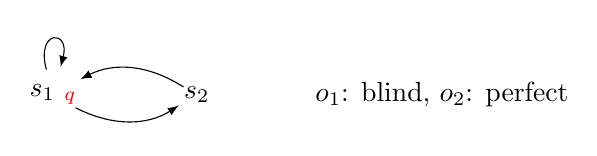
\begin{tikzpicture}[%
      every node/.style={circle,minimum size=4pt,minimum height=4pt, inner sep=0pt},
      shorten >=2pt,
      node distance=1.3cm, >=latex
    ]
    \node [] (0) [circle] {$s_1~_{\color{red}q}$};
    \node [] (1) [circle, right=of 0] {$s_2$};
    \node [] (2) [rectangle, right=of 1] {$o_1$: blind, $o_2$: perfect}; 
    \path [draw] (0) edge[->, bend right]  node {} (1)
    (0) edge[->, loop above]  node {} (0)
    (1) edge[->, bend right]  node {} (0);
  \end{tikzpicture}
  \end{center}
  \hrule
  \begin{center}
  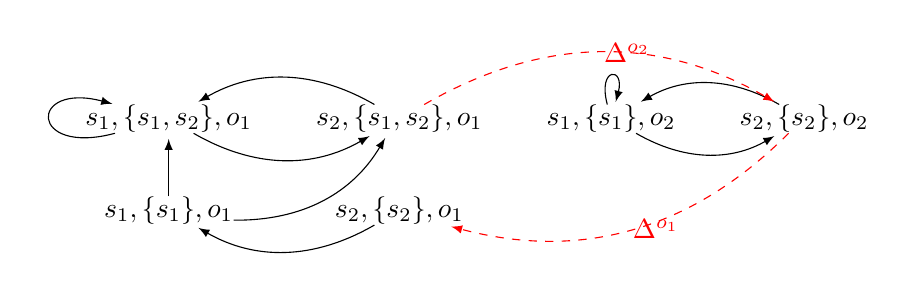
\begin{tikzpicture}[%
      every node/.style={circle,minimum size=4pt,minimum height=4pt, inner sep=0pt},
      shorten >=2pt,
      node distance=0.8cm, >=latex
    ]
    \node [] (0) [rectangle] {$s_1,\{s_1,s_2\},o_1$};
    \node [] (1) [rectangle, right=of 0] {$s_2,\{s_1,s_2\},o_1$};
    \node [] (2) [rectangle, below=of 0] {$s_1,\{s_1\},o_1$};
    \node [] (3) [rectangle, below=of 1] {$s_2,\{s_2\},o_1$};
    \node [] (4) [rectangle, right=of 1] {$s_1,\{s_1\},o_2$};
    \node [] (5) [rectangle, right=of 4] {$s_2,\{s_2\},o_2$};
    \path [draw] (0) edge[->, bend right]  node {} (1)
    (0) edge[->, loop left]  node {} (0)
    (1) edge[->, bend right]  node {} (0)
    (4) edge[->, bend right]  node {} (5)
    (4) edge[->, loop above]  node {} (4)
    (5) edge[->, bend right]  node {} (4)
    (2) edge[->]  node {} (0)
    (2) edge[->, bend right]  node {} (1)
    (3) edge[->, bend left]  node {} (2)
    (1) edge[dashed, ->, bend left, color=red,right] node {$\D{o_2}$} (5)
    (5) edge[dashed, ->, bend left, color=red,right] node {$\D{o_1}$} (3)
    ;
  \end{tikzpicture}
  \end{center}
\end{frame}


\begin{frame}{Example}
  $$\varphi=\D{o_2}(\K q\vee\neg q)$$
  \vfill
    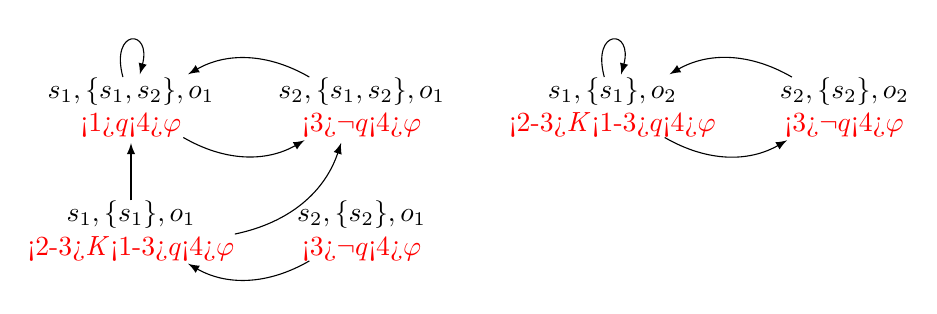
\begin{tikzpicture}[%
      every node/.style={circle,minimum size=4pt,minimum height=4pt, inner sep=0pt},
      shorten >=2pt,
      node distance=0.8cm, >=latex
    ]
    \node [] (0) [rectangle, align=center] {$s_1,\{s_1,s_2\},o_1$\\\color{red}{\onslide<1>{$q$}}{\onslide<4>{$\varphi$}}};
    \node [] (1) [rectangle, right=of 0, align=center] {$s_2,\{s_1,s_2\},o_1$\\\color{red}{\onslide<3>{$\neg q$}}{\onslide<4>{$\varphi$}}};
    \node [] (2) [rectangle, below=of 0, align=center] {$s_1,\{s_1\},o_1$\\\color{red}{\onslide<2-3>{$\K$}}{\onslide<1-3>{$q$}}{\onslide<4>{$\varphi$}}};
    \node [] (3) [rectangle, below=of 1, align=center] {$s_2,\{s_2\},o_1$\\\color{red}{\onslide<3>{$\neg q$}}{\onslide<4>{$\varphi$}}};
    \node [] (4) [rectangle, right=of 1, align=center] {$s_1,\{s_1\},o_2$\\\color{red}{\onslide<2-3>{$\K$}}{\onslide<1-3>{$q$}}{\onslide<4>{$\varphi$}}};
    \node [] (5) [rectangle, right=of 4, align=center] {$s_2,\{s_2\},o_2$\\\color{red}{\onslide<3>{$\neg q$}}{\onslide<4>{$\varphi$}}};
    \path [draw] (0) edge[->, bend right]  node {} (1)
    (0) edge[->, loop above]  node {} (0)
    (1) edge[->, bend right]  node {} (0)
    (4) edge[->, bend right]  node {} (5)
    (4) edge[->, loop above]  node {} (4)
    (5) edge[->, bend right]  node {} (4)
    (2) edge[->]  node {} (0)
    (2) edge[->, bend right]  node {} (1)
    (3) edge[->, bend left]  node {} (2)
    ;
  \end{tikzpicture}
    \vfill
    \textbf{Subformula:}
    \onslide<4>{$\D{o_2}($}\onslide<2,4>{$\K$}\onslide<1-2,4>{$q$}\onslide<4>{$\vee$}\onslide<3-4>{$\neg q$}\onslide<4>{$)$}\\
    
\end{frame}


\begin{frame}{Algorithm}
  \footnotesize
  \begin{block}{While there exists $\D{o}\varphi$ or $\K\varphi$ subformula ($\varphi$ \ctls\ formula)}
    Mark the states where $\varphi$ holds using a \ctls\ model-checker, with a new atomic proposition $p_{\varphi}$.\\
    If the subformula is $\K\varphi$, mark with a new atomic proposition $p_\phi$ every $(I,s,o)$ such that $\forall s'\in I, (I,s',o)$ has been marked with $p_{\varphi}$.\\
    If the subformula is $\D{o}\varphi$, mark with a new atomic proposition $p_\phi$ every $(I,s,o')$ such that $(\UD(I,s,o),s,o)$ has been marked with $p_{\varphi}$.\\
    Replace $\K\varphi$ or $\D{o}\varphi$ with $p_\phi$.
  \end{block}
  \vfill
  \begin{exampleblock}{When there is no more $\K$ or $\D{o}$}
    The final formula is a \ctls\ formula with new atomic propositions.
    It can be model-checked with a \ctls\ model-checker.
  \end{exampleblock}
    

\end{frame}



%\metroset{sectionpage=none}
\section{Conclusion}
We successfully defined a logic to capture the dynamic changes of observation. We introduced an alternative semantics that we proved to be equivalent and is easier to model-check. This logic can be model-checked using a marking algorithm. We have shown that it can be extended to multi-agent settings with nested knowledge operators using the \ktree\ structure defined in~\cite{DBLP:conf/fsttcs/MeydenS99}.

We believe that our work could be insightful for future works on Strategy Logic with Imperfect Information~\cite{DBLP:conf/lics/BerthonMMRV17}\cite{epistemicSL}, and provide elements for model-checking epistemic extensions.

Another possible future work could be extending \ctlskd. Allowing $\D{o}\psi$ to be a path formula instead of a history formula would define a logic that we suspect to be more expressive than \ctlskd.
We haven't solved the model-checking problem for this extension yet. The marking algorithm cannot be applied anymore because $\D{o}\psi$ cannot be marked on the states of the augmented model, as it also requires a run to be interpreted.
 We believe that we could define a \textit{focus game}, as defined in~\cite{DBLP:journals/logcom/LangeS02}. These games are defined such that there exists a winning strategy for some player if and only if a model satisfy a given formula. This work has yet to be done.


\end{document}
